\documentclass[../main.tex]{subfiles}

\begin{document}

\begin{figure}
    \centering
    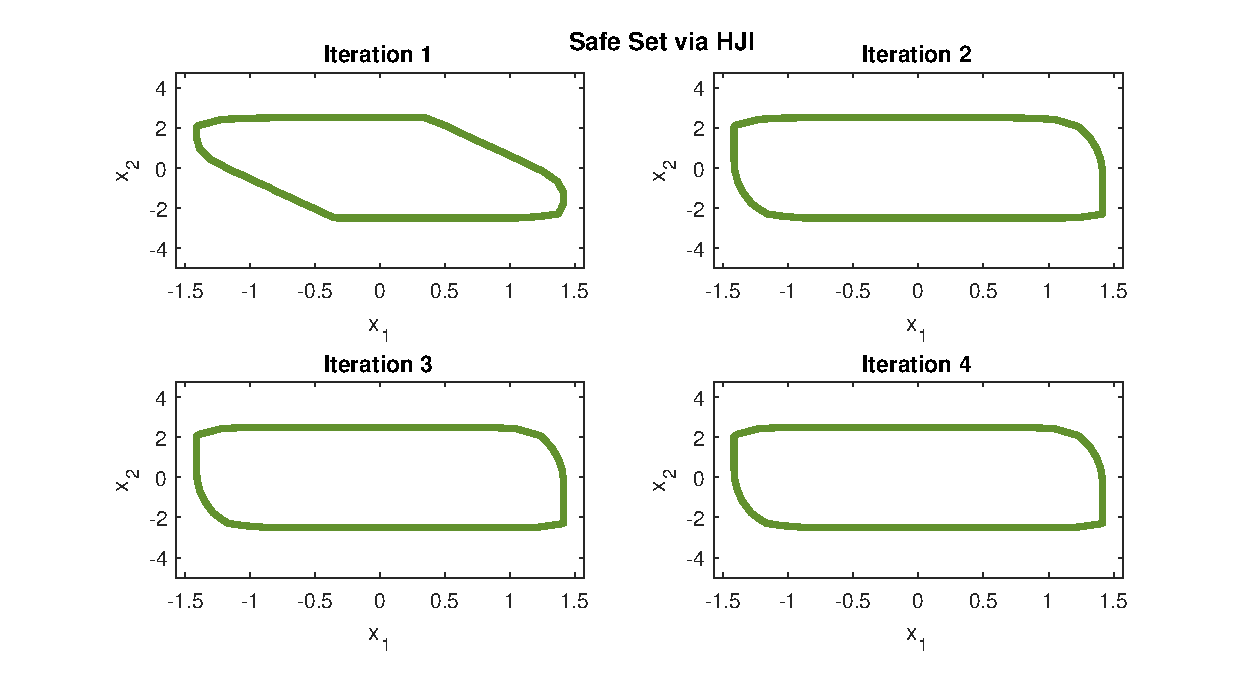
\includegraphics[width=\textwidth]{SafeSet_it4_unexplore}
        \caption{Safe Set Computation in four iterations. Clearly, the safe set already converges after the first iteration.}  \label{fig:SafeSet_it4_unexplore}
\end{figure}

\begin{figure}
    \centering
    \makebox[\textwidth][c]{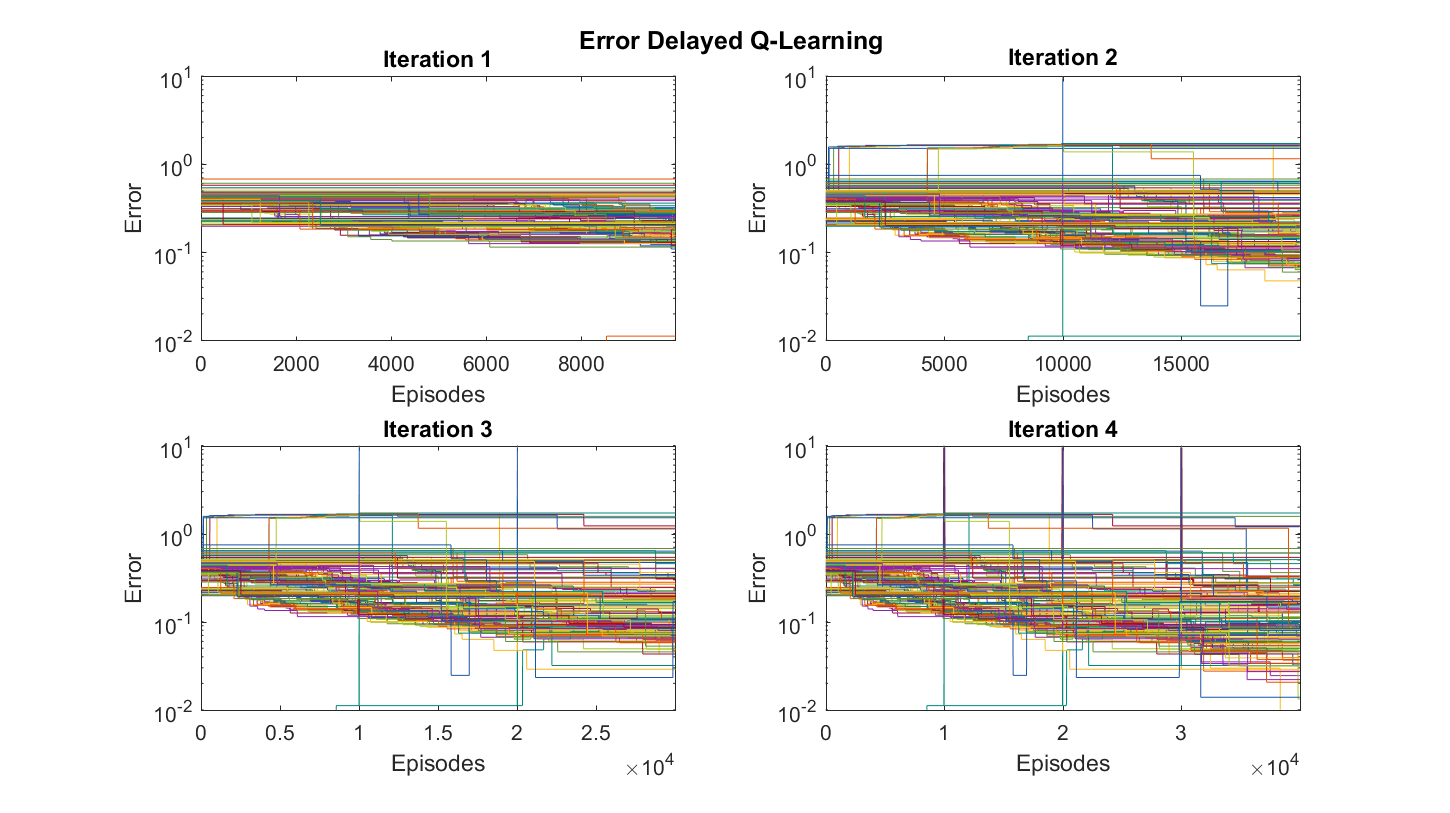
\includegraphics[width=1.2\textwidth]{Learning_it4_unexplore}}
        \caption{Logarithmic Error of the learned values compared to the values computed by Value Iteration. Each iteration consists of $10000$ steps.}  \label{fig:Learning_it4_unexplore}
\end{figure}

\begin{figure}
    \centering
    \makebox[\textwidth][c]{\includegraphics[width=1.2\textwidth]{GP_it4_unexplore}}
        \caption{Gaussian Process regression in four iterations.}  \label{fig:GP_it4_unexplore}
\end{figure}

\begin{figure}
    \centering
    \makebox[\textwidth][c]{\includegraphics[width=1.2\textwidth]{GP_it4_explore}}
        \caption{Gaussian Process regression in four iterations with incremental Q-learning.}  \label{fig:GP_it4_explore}
\end{figure}

\iffalse
\begin{figure}
    \centering
    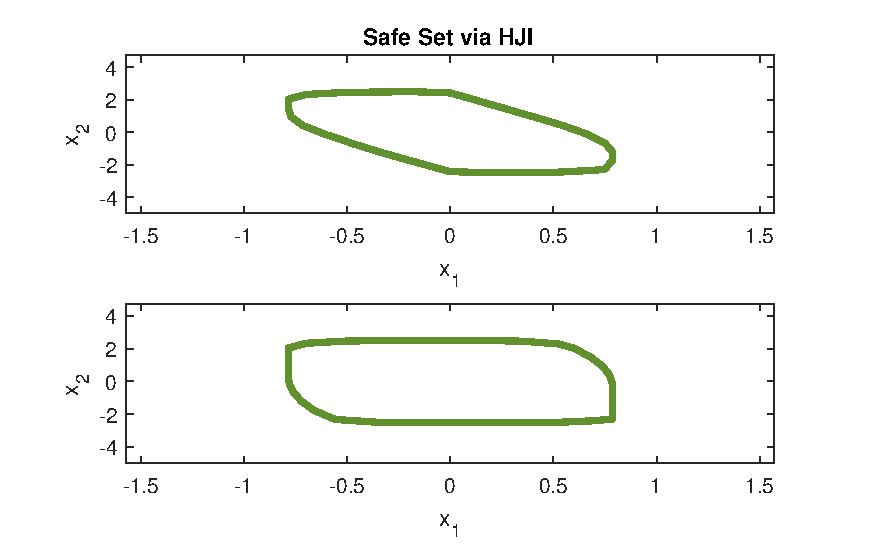
\includegraphics[width=\textwidth]{SafeSet}
        \caption{Safe Set Computation.}  \label{fig:SafeSet}
\end{figure}

\begin{figure}
    \centering
    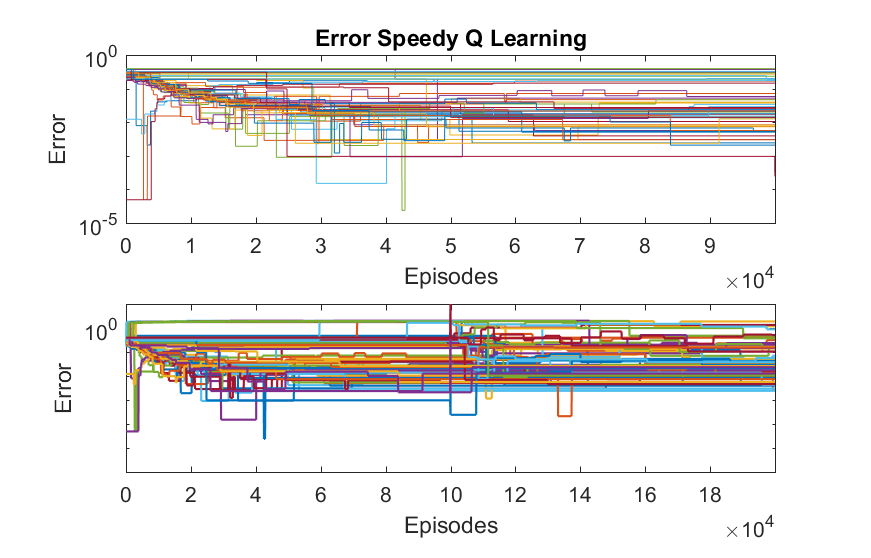
\includegraphics[width=\textwidth]{Learning}
        \caption{Choice of samples (red) by employing a grid (blue) and taking the nearest neighbours to the grid points in order to ensure that the samples cover the whole state space.}  \label{fig:Learning}
\end{figure}

\begin{figure}
    \centering
    \includegraphics[width=\textwidth]{GP}
        \caption{Choice of samples (red) by employing a grid (blue) and taking the nearest neighbours to the grid points in order to ensure that the samples cover the whole state space.}  \label{fig:GP}
\end{figure}

\begin{figure}
    \centering
   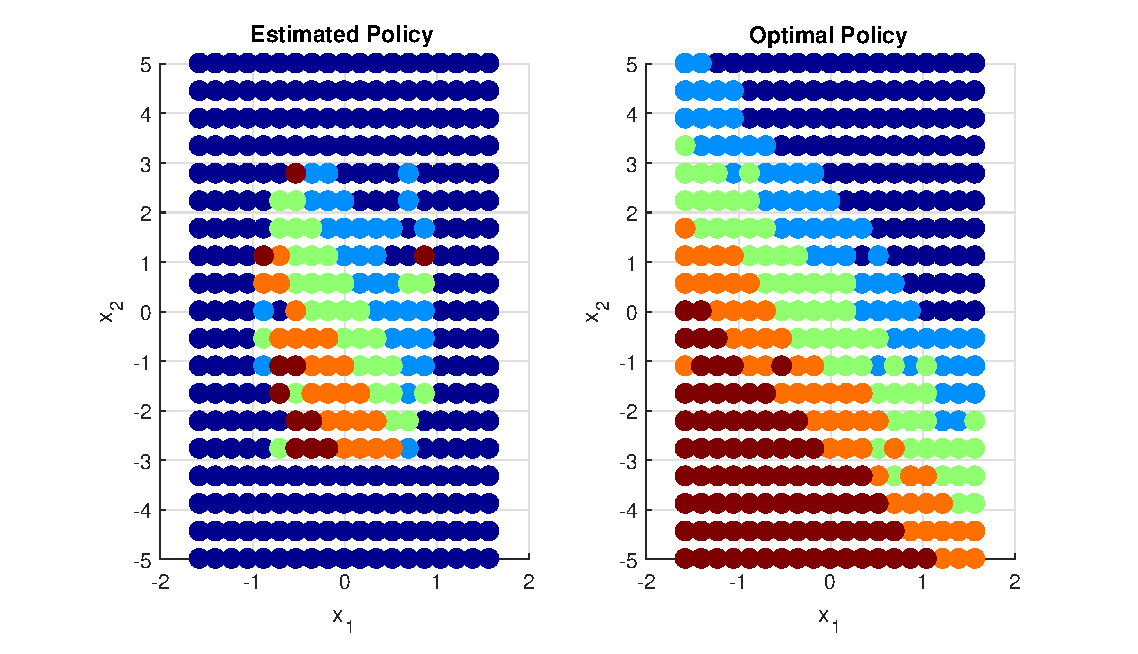
\includegraphics[width=\textwidth]{Policy}
        \caption{Choice of samples (red) by employing a grid (blue) and taking the nearest neighbours to the grid points in order to ensure that the samples cover the whole state space.}  \label{fig:Policy}
\end{figure}

\begin{figure}
    \centering
    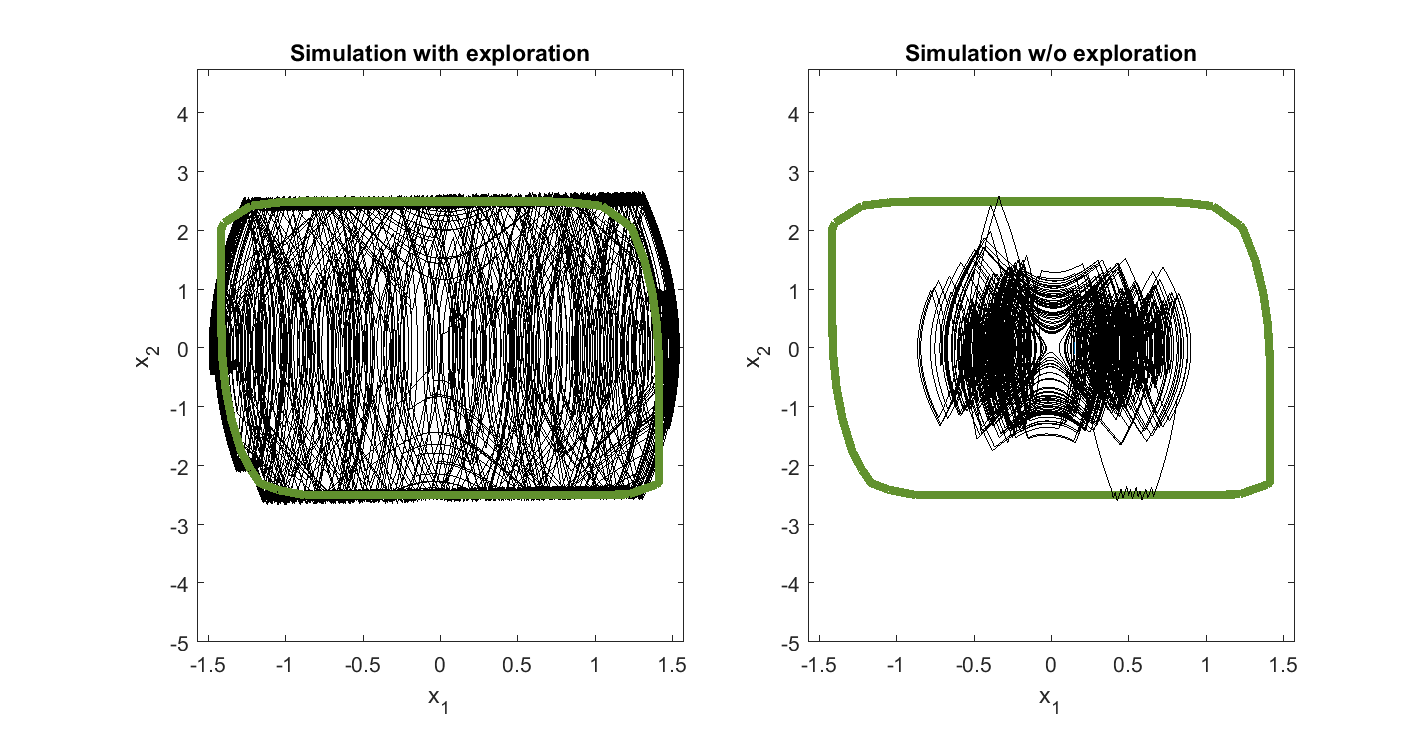
\includegraphics[width=\textwidth]{Simulation}
        \caption{Choice of samples (red) by employing a grid (blue) and taking the nearest neighbours to the grid points in order to ensure that the samples cover the whole state space.}  \label{fig:Simulation}
\end{figure}

\begin{itemize}
    \item Convergence of Policy
    \item Safe Set 
    \item Estimated Disturbance
    \item Overall Performance in Simulations
    \item comparison to Wang
\end{itemize}
\fi

\begin{figure}
    \centering
    \begin{subfigure}[b]{\textwidth}
    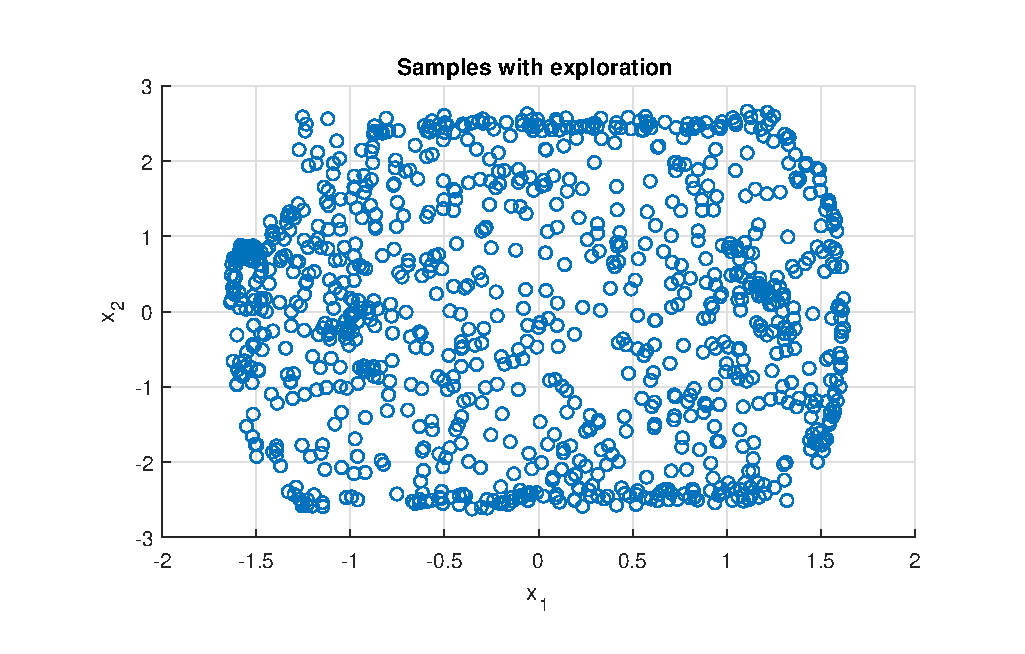
\includegraphics[width=\textwidth]{samples_exploration}
    \end{subfigure}
    
    \begin{subfigure}[b]{\textwidth}
    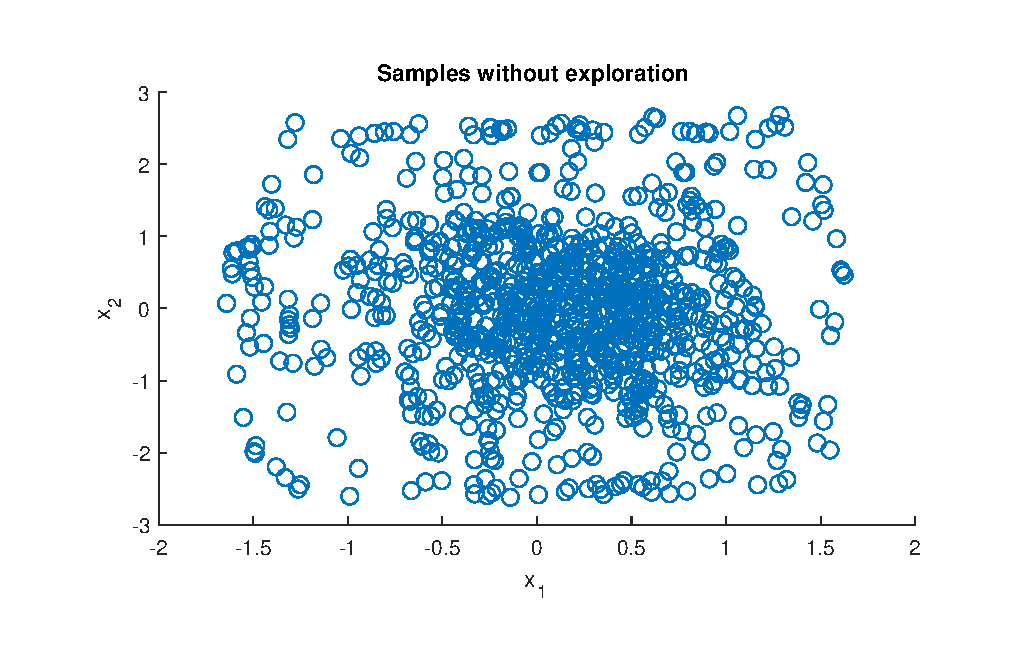
\includegraphics[width=\textwidth]{samples_unexploration}
    \end{subfigure}
        \caption{Random sampling with and without incremental Q-learning. In the upper figure, the spread of the samples is clearly better, whereas in the lower figure most samples are concentrated around the origin.}  \label{fig:samples_exploration}
\end{figure}


\begin{figure}
    \centering
    \makebox[\textwidth][c]{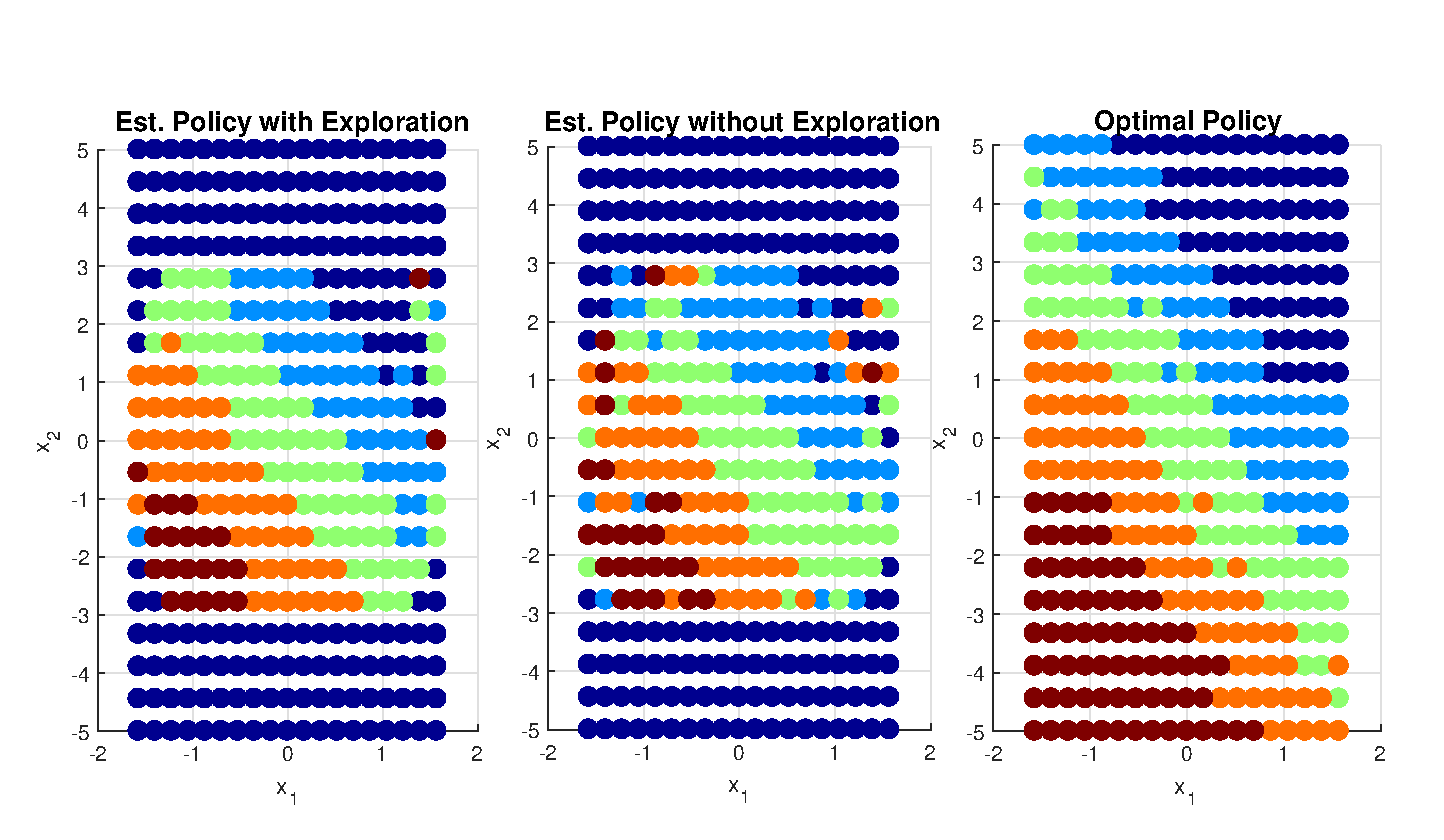
\includegraphics[width=1.2\textwidth]{policy_exploration}}
    \caption{Policy estimation with and without exploration. After the same number of learning iterations, the algorithm with exploration achieves considerably better results above all at the edges of the safe set.} \label{fig:policy_exploration}
\end{figure}
\end{document}